% !TeX root = article.tex
\section{Description of plasticity in the framework of physics engine}

In this section, key concepts related to the introduced model are explained. Main differences between 
traditional structural analysis and physics engines are reviewed and discussed.

Velocity-based formulation is  popular within physics based game
developers and film production teams.
%\citet[p.~45]{erleben.thesis} 
\citet{erleben.thesis} 
provides reasoning and theoretical details on why 
velocity-based formulation is  popular in constraint-based rigid body simulation. 
Main reason is that collision handling can be done without additional procedures.

Background
for velocity based formulation shown here is based on  
\citet{erleben.thesis}.
%\citet[p.~45-50]{erleben.thesis}.
% pdf page 64
In following section, these formulations will be clarified by simple example using \bullet\ implementation.

Impulse $\vec{J}$
in the time interval $\Delta t $ can we written as
\begin{equation} \label{eq:impulseIntegral}
\vec{J} = \int_{0}^{\Delta t} \vec{f}_{true}(t) dt
\end{equation}
where $\vec{f}_{true}(t)$ is force.

Newton's second law of motion $\vec{F}=m\vec{a}$ one can solve for the velocity,
$\vec{v}^{\Delta t}$ as
\begin{equation} \label{eq:impulseIntegraWithNewton}
\int_{0}^{\Delta t} m \frac{d\vec{v}}{dt}dt= \int_{0}^{\Delta t} \vec{f}_{true}(t)
\end{equation}
\begin{equation} \label{eq:impulse}
m(\vec{v}^{\, \Delta t} - \vec{v}^{\, 0})=\vec{J}
\end{equation}
where superscripts denote time, i.e. ${\vec{v}}^{\Delta t}=\vec{v}(\Delta t)$.
Next position can be found
by integrating the velocity.
Updates after each step can be summarized  for locations and  
for velocities correspondingly as follows.

\begin{equation} \label{eq:eomL} % pdf page 69
\vec{s}^{\, t+\Delta t} = \vec{s}^{\, t}+\Delta t S \vec{u}^{\, t+\Delta t}
\end{equation}

\begin{equation} \label{eq:eomV}
\vec{u}^{\, t+\Delta t} = \vec{u}^{\, t}+\Delta t M^{-1}(C N \vec{f}^{\ t+\Delta t} + \vec{f}_{ext}) 
\end{equation}

Symbols used in Equations \ref{eq:eomL} and \ref{eq:eomV}
are summarized in Table \ref{tab:eom} and Figure \ref{fig:eom-contact}.
Figure \ref{fig:eom-contact} describes collision of two bodies $B_1$ and $B_2$

\begin{figure}[htb!]
\centering
\begin{tikzpicture}
\coordinate (O1) at(2,1);
\coordinate (O2) at(2,4);
\coordinate (C) at(2,2);
\draw (0,0) -- (4,0) -- (4,2) -- (0,2) --(0,0);
\draw (2,2) -- (3.5,5) -- (0.5,5) -- (2,2) ;
\node at (3.5,0.4) {$B_1$};
\filldraw (O1) circle (0.5mm) node[anchor=north] {$\vec{r}_1$};
\node at (2.8,4.5) {$B_2$};
\filldraw (O2) circle (0.5mm) node[anchor=south] {$\vec{r}_2$};
\filldraw (C) circle (0.5mm) node[anchor=north west] {$\vec{p}_1$};
\draw[-{Stealth[length=3mm]}] (O1) -- (C) node[anchor=north east] {$\vec{r}_{11}$};
\draw[-{Stealth[length=3mm]}] (O2) -- (C) node[anchor=south east] {$\vec{r}_{21}$};
\draw[-latex,thick] (C) -- ++(0,1.4) node[anchor=west] {$\vec{n}_{1}$};
\node[anchor=west] at (4.5,4.5) {
$\vec{r}_i$  =  orientation of body $i$
};
\node[anchor=west] at (4.5,4) {$\vec{p}_k $ = orientation of contact point $k$};
\node[anchor=west] at (4.5,3.5) {$\vec{r}_{ik} $ = $\vec{p}_k - \vec{r}_i $};
\node[anchor=west] at (4.5,3) {$\vec{n}_{k} $ = normal for contact point $k$};
\end{tikzpicture}
\caption{Illustration of nomenclature for equations of motion for contact.}
\label{fig:eom-contact}
\end{figure}

where $\vec{r}_i$ is orientation of body $i$,
$\vec{p}_k $ is orientation of contact point $k$,
$\vec{r}_{ik} $ is vector  between center of gravity of body $i$ and contact point $k$
and
$\vec{n}_{k}$ is contact normal for contact point $k$.
By employing this formulation, simplified scenario can be simulated.


% pdf page 33, notation in typical ODEs
\begin {table}[htb!]
\caption {Nomenclature for equations of motion}
\label{tab:eom}
\begin{center}
\begin{tabular}{|l| l|}
\hline
{\bf Symbol} & {\bf Description} \\  \hline
$\vec{r}_i$ & position of center of mass for body $i$  \\ \hline
$\vec{q}_i$ & orientation for body $i$ as quaternion $\lbrack s_i, x_i, y_i, z_i \rbrack ^T $ \\
\hline
$\vec{p}_h$ & contact or joint point $k$  \\ \hline
$\vec{r}_{ki}$ & $\vec{p}_k - \vec{r}_i$  \\ \hline
$\vec{s}$ & $\lbrack \vec{r}_1, \vec{q}_1,...,\vec{r}_n, \vec{q}_n \rbrack ^T $\\ \hline
$Q_i$ & \begin{tabular}{@{}c}
rotation of quaternion $\vec{q}_i$
as matrix \\ where 
$\frac{1}{2}\vec{\omega}_i \vec{q}_i=Q_i \vec{\omega}_i$
\end{tabular}
   $
\frac{1}{2} \left[ \begin{array}{ccc}
-x_i & -y_i & -z_i \\
s_i & z_i & -y_i \\
-z_i & s_i & x_i \\
y_i & -x_i & s_i
\end{array} \right]
$
\\ \hline
$S$ & 
\begin{tabular}{@{}c}
generalized transformation matrix \\
$ S \in \mathbb{R}^{7n \times 6n}$
\end{tabular}
 $ \left[ \begin{array}{ccccc}
1 &  &  & & 0 \\
 & Q_i  \\
 & & \ddots  \\
 & & & 1 \\
0 & & & & Q_n 
\end{array} \right]
$
\\ \hline
$\vec{v}_i$ & linear velocity of  center of mass for body $i$   \\ \hline
$\vec{\omega}_i$ & angular velocity of center of mass for body $i$  \\ \hline
$\vec{u}$ & $\lbrack \vec{v}_1, \vec{\omega}_1,...,\vec{v}_n, \vec{\omega}_n \rbrack ^T $\\ \hline
$M$ &
\begin{tabular}{@{}c}
 generalized mass matrix \\
$ M \in \mathbb{R}^{6n \times 6n}$  
\end{tabular}
$
\left[ \begin{array}{ccccc}
m_i 1 &  &  & & 0 \\
 & I_1  \\
 & & \ddots  \\
 & & & m_n 1 \\
0 & & & & I_n 
\end{array} \right]
$
\\ \hline
$I_i$ & inertia tensor for body $i$  \\ \hline
$C$ & contact condition matrix  $ C \in \mathbb{R}^{6n \times 3K}$ \\ \hline
$N$ & contact normal matrix  $ N \in \mathbb{R}^{3K \times K}$ \\ \hline
\end {tabular}
\end{center}
\end {table}

Friction in contacts and joint constraints can be handled in unified way by refactoring
equation \ref{eq:eomV} as,  
\citet{erleben.thesis}
%\citet[p.~66-67]{erleben.thesis}
\begin{equation} \label{eq:eomV2}
\vec{u}^{\, t+\Delta t} = \vec{u}^{\, t}+\Delta t M^{-1}(
 J_{contact}^T \vec{\lambda}_{contact}
+ J_{joint}^T \vec{\lambda}_{joint}
+ \vec{f}_{ext})
\end{equation}

where jacobian terms $J_{contact}^T$ for joints are 
derived by taking time derivates of kinematic constraints.

Symbols used in Equation \ref{eq:eomV2} are summarized in Table
\ref{tab:eom-g} and Figure \ref{fig:eom-joint}.
Figure \ref{fig:eom-joint} shows terms needed for joint processing.

\begin{figure}[htb!]
\centering
\begin{tikzpicture}
\coordinate (O1) at(1,1);
\coordinate (O2) at(1,3);
\coordinate (C) at(1,2);
\draw (0,0) -- (2,0) -- (2,2) -- (0,2) --(0,0);
\draw (0,2) -- (2,2) -- (2,4) -- (0,4) --(0,2) ;
\node at (0.5,0.4) {$B_1$};
\filldraw (O1) circle (0.5mm) node[anchor=north] {$\vec{r}_1$};
\node at (0.5,3.5) {$B_2$};
\filldraw (O2) circle (0.5mm) node[anchor=south] {$\vec{r}_2$};
\draw[-{Stealth[length=3mm]}] (O1) -- (C) node[anchor=north east] {$\vec{r}_{anc}^{\,1}$};
\draw[-{Stealth[length=3mm]}] (O2) -- (C) node[anchor=south east] {$\vec{r}_{anc}^{\,2}$};
\node[anchor=west] at (4.5,3.5) {
$\vec{r}_i$  =  orientation of body $i$ 
};
\node[anchor=west] at (4.5,3) {$\vec{r}_{anc}^{\,i} $ = body frame vector $i$};
\end{tikzpicture}
\caption{Illustration of nomenclature for equations of motion for joint.}
\label{fig:eom-joint}
\end{figure}

In Figure \ref{fig:eom-joint}, $\vec{r}_{anc}^{\,i}$ is used to define at which point
joint constraint is applied.

% pdf page 33, notation in typical ODEs
\begin {table}[htb!]
\caption {Additional terms  for generalized equations of motion}
\label{tab:eom-g}
\begin{center}
\begin{tabular}{|l| l|}
\hline
{\bf Symbol} & {\bf Description} \\  \hline
$J_{contact}$ & Jacobian matrix for contacts  \\ \hline
$\lambda_{contact}$ & vector of lagrange multipliers for contacts  \\ \hline
$J_{joint}$ & Jacobian matrix for joints  \\ \hline
$\lambda_{joint}$ & vector of lagrange multipliers for joints  \\ \hline
\end {tabular}
\end{center}
\end {table}

Constraint processing in \bullet\ is based on ODE, \cite{ode}.
Joints are also discussed in detail in  
\citet{erleben.thesis}.
%\citet[p.~60-90]{erleben.thesis}.
Equations \ref{eq:constraintEquation}, \ref{eq:lambdaLow} and
\ref{eq:lambdaHigh} 
are created for each constraint. 
Derivation for terms in Equation \ref{eq:constraintEquation}
can be done using position and orientation of connected bodies.
E.g. for ball joint formulation is based on both joint points having same position.
In contact cases formulation is easier if it is done using velocities, \cite{ode.joints}.

\begin{equation} \label{eq:constraintEquation}
J_1 \vec{v}_1 + \Omega_1 \vec{\omega}_1 + 
J_2 \vec{v}_2 + \Omega_2 \vec{\omega}_2 = \vec{c} + C \vec{\lambda}
\end{equation}

\begin{equation} \label{eq:lambdaLow}
\vec{\lambda} \geq \vec{l}
\end{equation}

\begin{equation} \label{eq:lambdaHigh}
\vec{\lambda} \leq \vec{h}
\end{equation}

In following section, these equations will be clarified by simple example.
Main parameters  and corresponding fields in \bullet\  
 are described in Table \ref{tab:constraintParameters}.

\begin {table}[htb!]
\caption {Constraint parameters}
\label{tab:constraintParameters} 
\begin{center}
\begin{tabular}{|c| l| l|}
\hline
{\bf Parameter} & {\bf Description} & {\bf btConstraintInfo2 pointer}\\  \hline
$J_1, \Omega_1$ & jacobian & m\_J1linearAxis, m\_J1angularAxis \\
$J_2, \Omega_2$ & & m\_J2linearAxis, m\_J2angularAxis \\ \hline
$\vec{v}$ & linear velocity & \\ \hline
$\vec{\omega}$ & angular velocity & \\ \hline
$\vec{c}$        &  right side vector   & m\_constraintError \\ \hline
$C$  & constraint force mixing & cfm \\  \hline
$\vec{\lambda}$ & constraint force &  \\ \hline
$\vec{l}$ & low limit for constraint force & m\_lowerLimit \\ \hline
$\vec{h}$ & high limit for constraint force & m\_upperLimit \\ \hline
\end {tabular}
\end{center}
\end {table}


In structural analysis, a formulation and associated numerical solution procedure are selected 
based on needed features.
Often,  finite element method is used.
In most cases, static solution with assumption of linear strain-displacement relation
using displacement based boundary conditions is used.
\citet{bathe-1975} provides description for handling of various nonlinearities.
In large displacement analysis, formulation may be based on updated formulation (Eulerian) or
Lagrangian formulation where initial configuration is used.
Further enhancements are material nonlinearity and dynamic analysis.
Physics engine provides dynamic analysis with large reference translations and rotations
while assuming bodies to be undeformable.

Material plasticity can be accounted in games by using suitable coefficient of restitution.
This provides reasonable means to simulate loss of energy in collisions.
Simulation of breaking of bodies made of ductile material can be made more realistic by splitting rigid body
to multiple bodies which are connected by energy absorbing joints.
Typical engineering stress-strain curve of ductile steel is shown in Figure \ref{fig:sscurve}.

\begin{figure}[htb!]
\centering
\begin{tikzpicture}
\coordinate (Y) at (1,4);
\draw[->] (0,0) -- (10,0) node[right] {\large{$\epsilon$}};
\draw[->] (0,0) -- (0,6) node[above] {\large{$\sigma$}};
\draw(0,0) -- (Y) -- (2,4) .. controls (7,6) .. (10,5);
\draw[dashed](0,4) -- (Y);
\node at (-0.2,4) [align=right] {$f_y$};
\draw(0.25,1) -- (0.5,1) -- (0.5,2);
\node at (0.75,1.5) {$E$};
\node at (0.8,2.5) [anchor=west] {$\sigma = E \epsilon$ if $\sigma \le f_y$};
\end{tikzpicture}
\caption{Engineering stress-strain curve of ductile steel (not to scale).}
\label{fig:sscurve}
\end{figure}

In Figure \ref{fig:sscurve}, $\sigma$ is stress, $E$ is Youngs modulus and $f_y$ is yield stress.
Engineering stress and strain mean that original dimensions are used in stress calculation,
\citet{dowling}.
%\citet[p.~108]{dowling}.
Stress-strain curve is not drawn to scale as elastic strain could not be seen as it is typically 0.001 to 0.005.

In this work elastic-fully plastic material model is used in most scenarios.
Having elastic part allows elastic displacements for slender structures. 
Elastic material behavior is ignored in approach introduced in this work provided
that deformation is related to higher frequency
than integration stability would allow.
It should be noted that geometry
of bodies is not updated during analysis and thus engineering stress-strain properties should
be used.

In this work, strain hardening is taken into account by assuming that plasticity in bending
expands, 
\citet{dowling}.
%\citet[p.~672]{dowling}.
Material that starts to yield first is hardened and as a result of which yielding moves.
This can be seen e.g. by bending paperclip. It does not break at low angles but can take few full bends. 

Difference between elastic and plastic section modulus is depicted in Figure \ref{fig:wp}.

\begin{figure}[htb!]
\centering
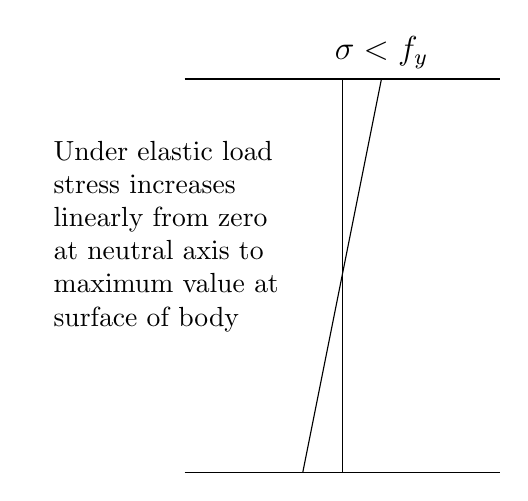
\begin{tikzpicture}
\coordinate (S) at (2.5,5);
\draw (0,5) -- (4,5) ;
\draw (0,0) -- (4,0) ;
\draw (2,0) -- (2,5) ;
\draw (1.5,0) -- (S); 
\node[above] at (S) [align=center] {\large{$\sigma<f_y$}};
\node[anchor=west] at (-2,3) {
\begin{tabular}{l}
Under elastic load\\
stress increases\\
linearly from zero\\
at neutral axis to\\
maximum value at \\
surface of body
\end{tabular}
};
\end{tikzpicture}
\hspace{1cm}
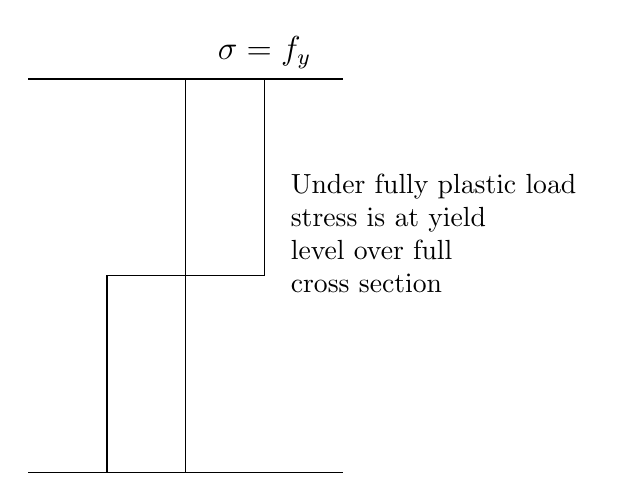
\begin{tikzpicture}
\coordinate (S) at (3,5);
\draw (0,5) -- (4,5) ;
\draw (0,0) -- (4,0) ;
\draw (2,0) -- (2,5) ;
\draw (1,0) -- (1,2.5) -- (3,2.5) -- (S); 
\node[above] at (S) [align=center] {\large{$\sigma=f_y$}};
\node[anchor=west] at (3,3) {
\begin{tabular}{l}
Under fully plastic load\\
stress is at yield\\
level over full\\
cross section
\end{tabular}
};
\end{tikzpicture}
\caption{Axial stress distribution over cross section for bending under elastic and fully plastic loads.}
\label{fig:wp}
\end{figure}

As shown in Figure 2.4, if stress is below yield limit $f_y$, stress and strain are linear within material.
If cross section is fully plastic, stress is assumed to be at yield level over whole cross section such that 
plastic section modulus is higher than elastic section modulus.

In this work, plasticity is handled by defining maximum forces
in Equations \ref{eq:lambdaLow} and  
\ref{eq:lambdaHigh} using plastic capasities which are defined below.

Maximum force acting in a direction of $\vec{r}_{anc}^{\,i} $
is product of area and yield stress as follows

\begin{equation} \label{eq:fN}
N_{max}= \int_A f_y
\end{equation}

Maximum forces acting perpendicular to $\vec{r}_{anc}^{\,i} $
are product of area and shear yield stress $\tau_y$ as follows
\begin{equation} \label{eq:fQ}
Q_{max}= \int_A \tau_y
\end{equation}

Maximum moments acting around axis perpendicular to $\vec{r}_{anc}^{\,i} $
are integrals of perpdendicular distance 
and yield stress $f_y$ as given for the moment around $x$-axis 
and moment around $z$-axis, respectively.

\begin{equation} \label{eq:Mx}
M_{max}^x= \int_A z f_y
\end{equation}

\begin{equation} \label{eq:Mz}
M_{max}^z= \int_A x f_y
\end{equation}

Maximum moment around $\vec{r}_{anc}^{\,i} $
is integral of distance $d$ from joint point
and shear yield stress $\tau_y$ as 

\begin{equation} \label{eq:My}
M_{max}^y= \int_A d \tau_y
\end{equation}

Maximum forces and moments for 
rectangular section with width $b$ and height $h$ using constant yield stress
are summarized in Table \ref{tab:maxForces}.
Yield shear stress is assumed to be $ 0.5\, f_y$ using Tresca yield critetion.
If von Mises yield criterion is used 0.5 is replaced by 0.58 ($1/\sqrt{3}$), \cite{dowling}.
% p. 262, p. 268
These are not exact values in multiaxial stress state but they
are usable in most cases.


\begin {table}[htb!]
\caption {Maximum forces and moments for 
rectangular section with width $b$ and height $h$ using constant yield stress $f_y$}
\label{tab:maxForces} 
\begin{center}
\begin{tabular}{| c| c|}
\hline
{\bf Direction} & {\bf Maximum value}  \\ \hline
maximum shear force & $0.5\, b\, h f_y$ \\ \hline
maximum normal force & $b\, h\, f_y$  \\ \hline
maximum bending moment in direction of $h$& $0.25\, b\, h^2 \, f_y$  \\ \hline
maximum bending moment in direction of $b$ & $0.25\, b^2\, h\, f_y$  \\ \hline
maximum torque & $ \approx 0.19\, b\, h\, \frac{b\, + h}{2} f_y$  \\ \hline
\end{tabular}
\end{center}
\end {table}

For torque there is closed form solution only for
circular cross sections.
Given approximation is 
best suited for cases where $b$ and $h$ are similar.
Better approximation for any given $b$ and $h$ can be obtained 
by integrating distance from center of joint over cross section and
multiplying it with yield shear stress e.g. using octave, \cite{octave}.
Example of calculation of maximum moment  around $\vec{r}_{anc}^{\,i} $
is shown in Figure \ref{fig:octave-mp}

\begin{figure}[htb!]
\centering
\lstset{language=octave}
\begin{lstlisting}
b=0.01; h=0.01; fy=200e6;
wpy=fy/2*dblquad(@(x,z) sqrt(x.*x+z.*z),-b/2,b/2,-h/2,h/2)
38.2
\end{lstlisting}

\caption{Calculation of maximum moment  around $\vec{r}_{anc}^{\,i} $ using octave.}
\label{fig:octave-mp}
\end{figure}


Basic idea introduced in this study can be tested with any framework having motors and hinge constraints.
This can be done by setting target velocity of motor to zero and limiting maximum motor impulse to plastic moment 
multiplied by timestep.

Further enhancements were created and tested by forking \bullet\ source code
and adding new constraints, \cite{pbullet}.
Instructions for using  windows executable and  source code are available, \cite{bp}.

